\begin{figure*}[t!]
    \centering
    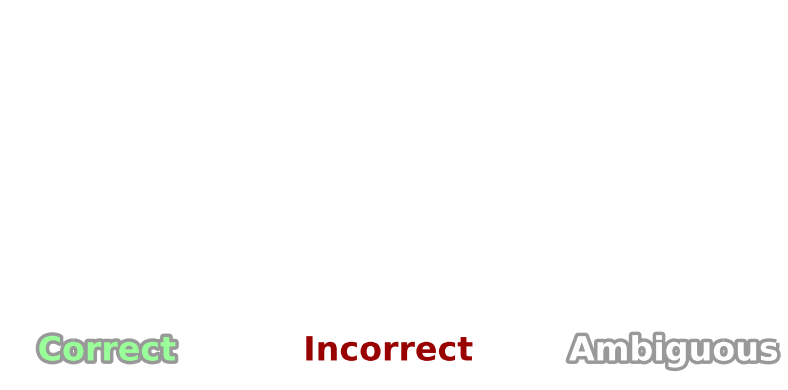
\includegraphics[width=0.5\textwidth, trim={0 0 0 3.3in},clip ] {figures/labels.png}\\
    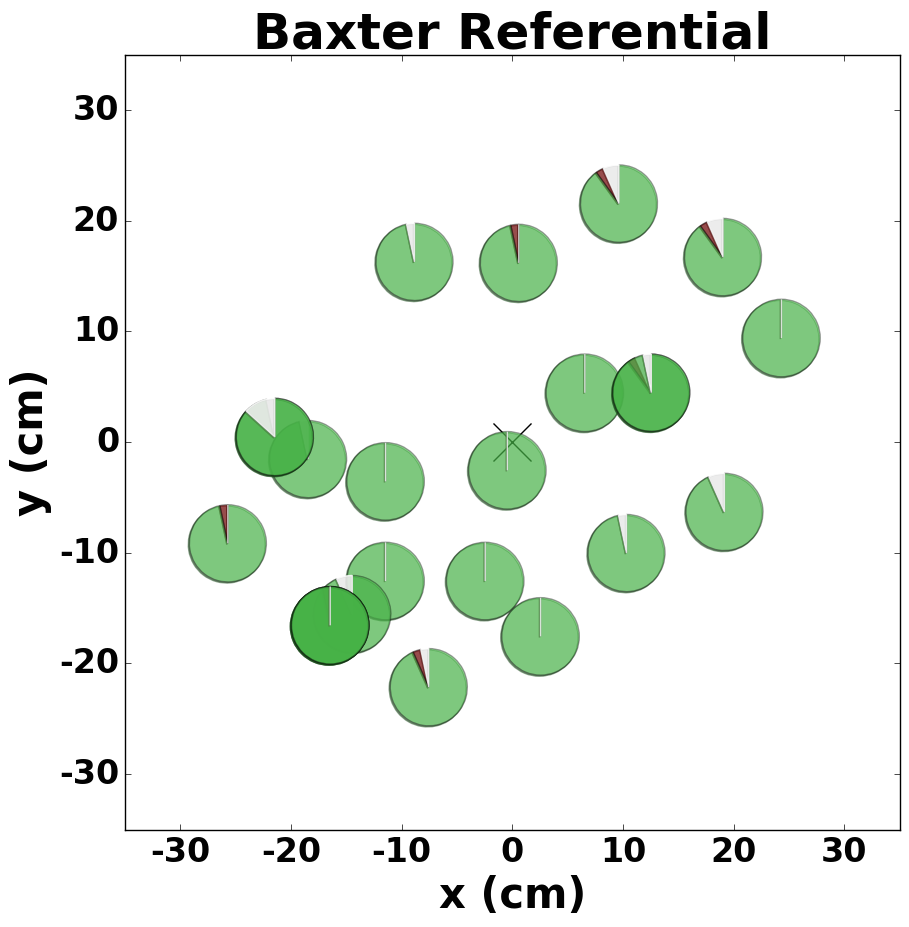
\includegraphics[width=0.32\textwidth ] {figures/baxter_Referential_.png}
    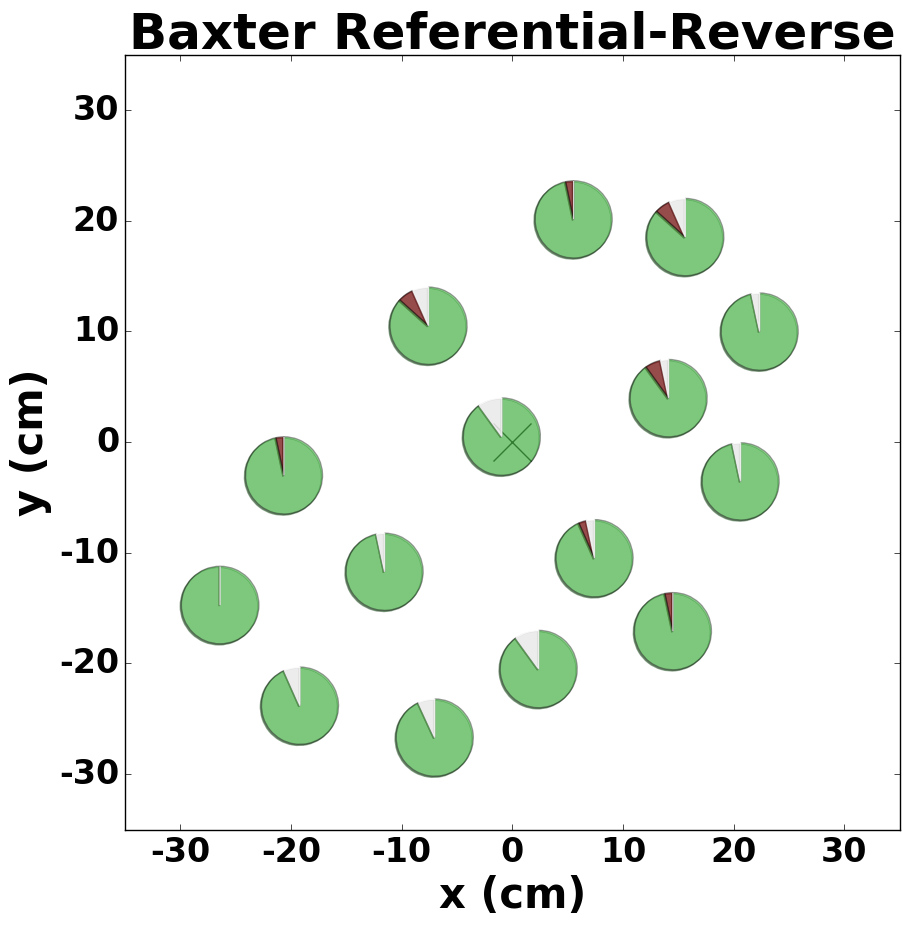
\includegraphics[width=0.32\textwidth ] {figures/baxter_Referential-Reverse_.png}
    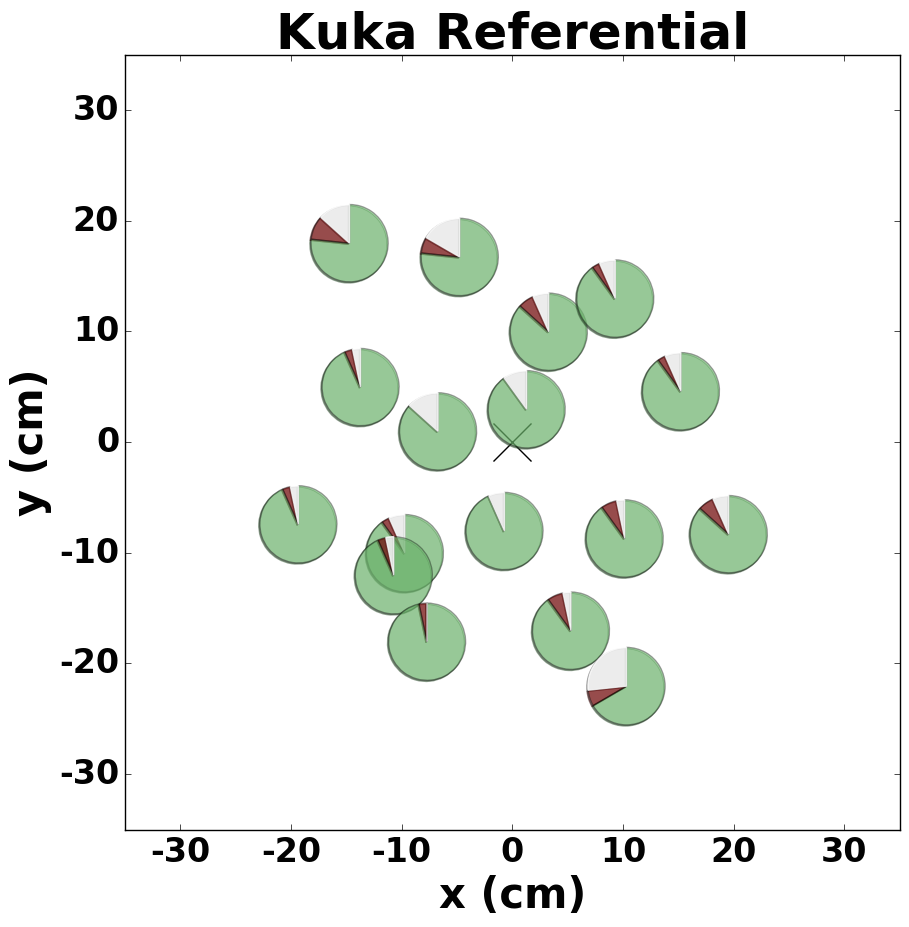
\includegraphics[width=0.32\textwidth ]{figures/kuka_Referential_.png}
    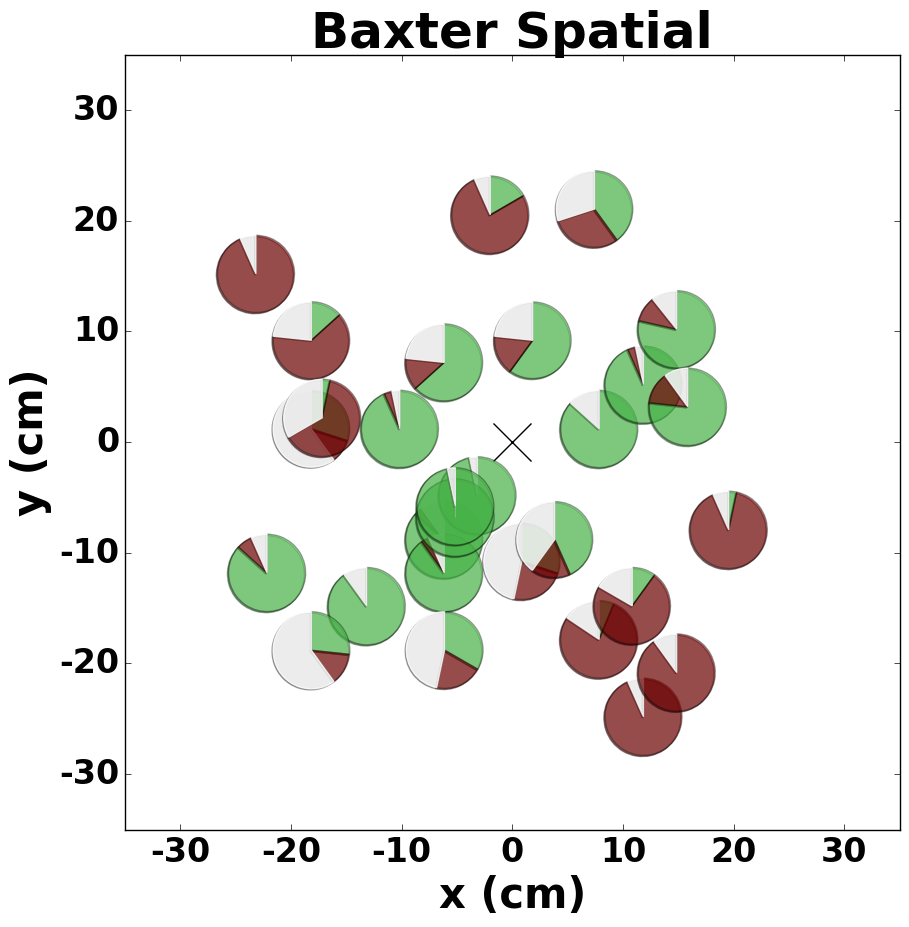
\includegraphics[width=0.32\textwidth ]{figures/baxter_Spatial_.png}
    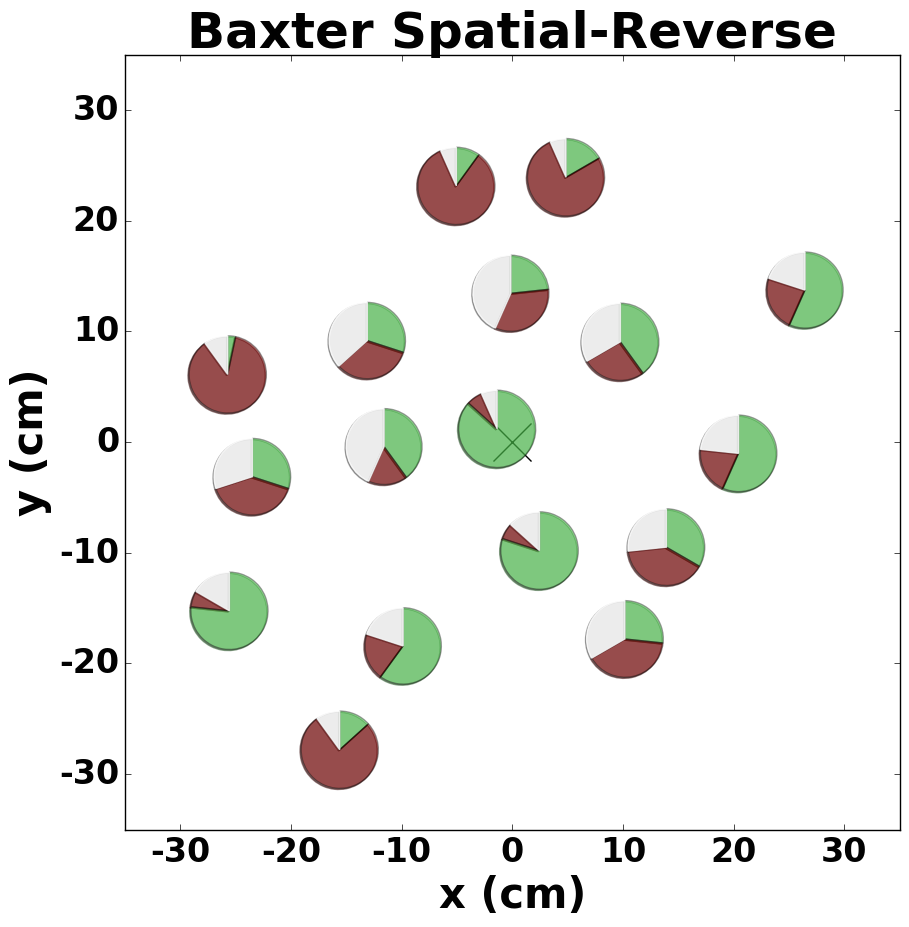
\includegraphics[width=0.32\textwidth ]{figures/baxter_Spatial-Reverse_.png}
    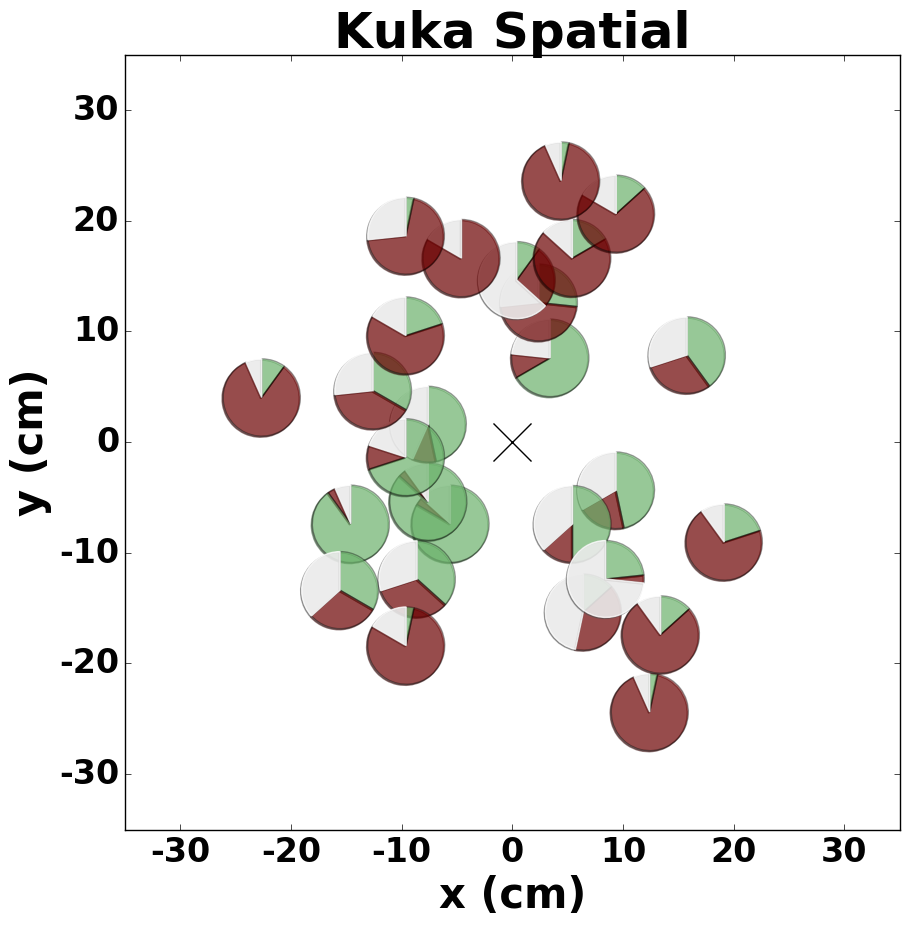
\includegraphics[width=0.32\textwidth ]{figures/kuka_Spatial_.png}
    \caption{The aggregated results from the referential versus spatial trials for the \textit{Baxter} and \textit{Kuka} robots. The locations of the responses correspond to the center of the circles, and are plotted in the coordinate frame centered at the position of the pointing action, marked with $\times$. The circles show the fraction of correct (grey), incorrect(black) and ambiguous(white) responses.}
    \label{fig:aggregatesimple}
\end{figure*}


% \begin{figure}[h]
%     \centering
%     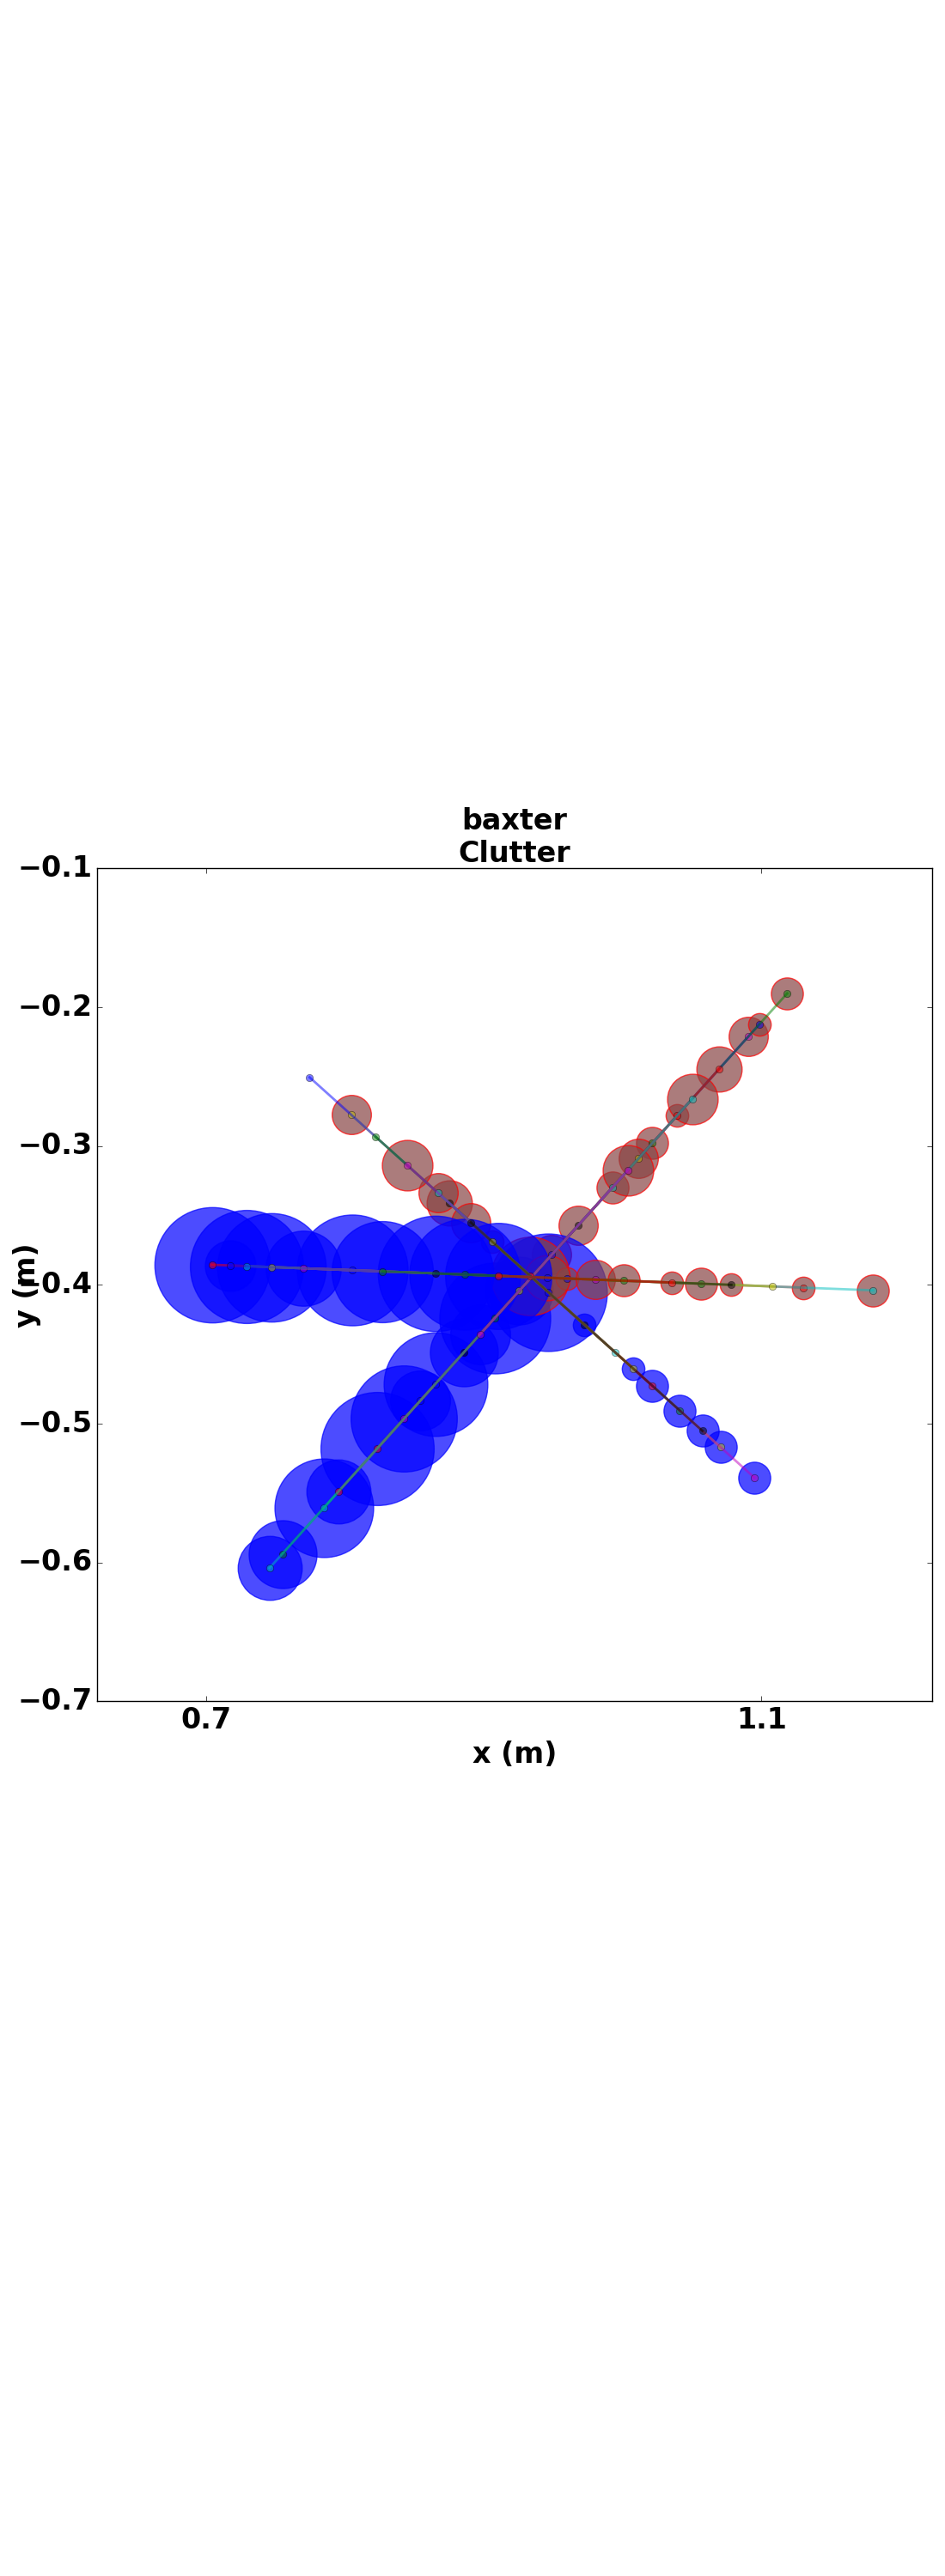
\includegraphics[width=0.47\textwidth ] {figures/baxter_Clutter_clutter.png}
%     \caption{The aggregated results from the cluttered scene trials for the \textit{Baxter} robot. The locations of the responses correspond to the center of the circles, and are plotted in the coordinate frame centered at the position of the true pointing action, marked with $\times$. Each circle shows the fraction of responses for cup 1 (red), and cup 2 (blue).}
%     \label{fig:baxterclutter}
% \end{figure}

\paragraph{Referential vs Spatial}
We study how varying the target of the pointing action from a referent object to a part of the space changes the interpretation of the pointing action by comparing the interpretation of the position of the pointing action $x^*$ in each condition. 
% $x^*$ represent the area on the table that contains the correct target of the pointing action. 


Figure~\ref{fig:aggregatesimple} shows the results of the experiment. The plot shows the spread of \textit{correct, incorrect, ambiguous} responses over the sampled positions about the location of a referential, and spatial pointing action. The referential data demonstrates the robustness of the interpretation. Most of the responses were overwhelmingly \textit{'correct'}, for both robots in interpreting a referent object in the \textit{pick} part of a pick-and-place task. The spatial pointing shows a much higher sensitivity to an accuracy of $x^*$ with respect to the true final placement. This comes up as a larger incidence of \textit{'incorrect'} and \textit{'ambiguous'} responses from the human subjects. This trend is true for the reverse trial as well.

While the study attempts to separate out and measure the critical aspects of the interpretation of robotic pointing actions some ambiguities like those arising out of perspective of the camera being projected onto a simulated 2D video or image are unavoidable. We suspect that the stretch of the 'correct' response green regions in the spatial plots is due to this perspective issue.

To test our hypothesis, we performed a Chi-squared test and compared the proportion of \textit{correct}, \textit{incorrect} and \textit{ambiguous} responses in referential and spatial trials. The results of the test shows that these two classes are statistically significantly different ($\chi^2= 13.89, p = 0.00096$).

To study if we are observing the same effects in the results of the reverse trial, no speech trial and the Kuka trial, we ran an equivalence test on the third hypothesis following the two one-sided tests method as described in \cite{lakens2017equivalence}, where each test is a pooled z-test with no continuity
correction with a significance level of 0.05. We found that changing the robot, removing the speech and the direction of the pointing action does not make a difference in the interpretation of spatial pointing and referential pointing within any margin that is less than 5\%.



\paragraph{Natural vs Unnatural}

We observed in the natural scene, when the end-effector points towards the edge of the cube that is on top of the stack, subjects place the new cube on top of the stack or on the table instead of the edge of the cube. However, in the unnatural scene, when we explain for subjects that there is no gravity, majority of them agree with the final image that has the cube placed on the edge of the cube. Table~\ref{tab:natural-unnatural} presents the results of this experiment. 

\begin{figure}[H]
% \vspace{-0.3in}
    \centering
    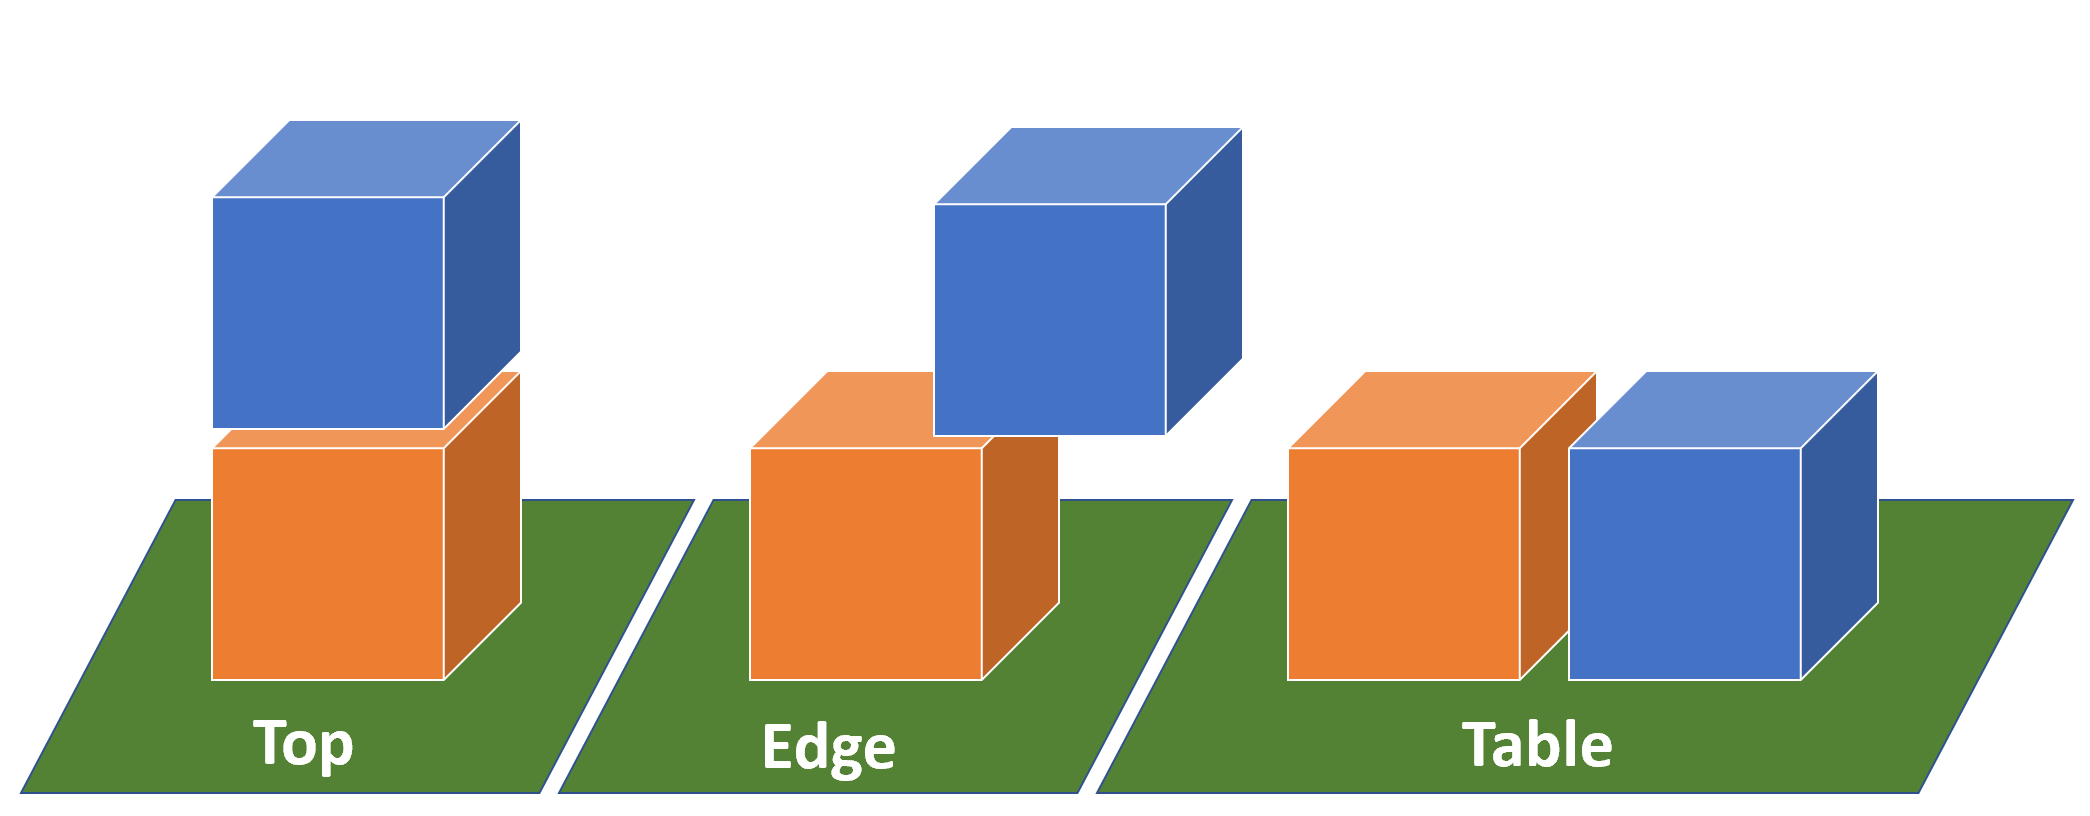
\includegraphics[width=0.4\textwidth, trim={0 0 0 0.7in},clip ] {figures/topedgetable.png}
    \vspace{-0.1in}
    \caption{
    The diagram shows the three different configurations of the placement of a blue cuboid object evaluated in the \textit{Natural vs Unnatural} trials. 
    % (\textit{Left:}) The object lies on top; (\textit{Middle:}) The object lies in an unstable manner off the edge;  (\textit{Right:}) The object lies beside on the table.
    }
    \label{fig:topedgetable}
    \vspace{-0.2in}
\end{figure}


\begin{table}[H]
\centering
\begin{tabular}{lllll}
& \multicolumn{1}{l}{} & \multicolumn{1}{l}{correct} & \multicolumn{1}{l}{incorrect} & ambiguous \\ \hline
\multicolumn{1}{l}{\multirow{unnatural}} & top                   & 12                           & 9                              & 9         \\
\multicolumn{1}{l}{}                           & \textbf{edge}                  & \textbf{24}                           & 2                              & 4         \\
\multicolumn{1}{l}{}                           & table                 & 2                            & 2                              & 26        \\ \hline
\multicolumn{1}{l}{\multirow{natural}}   & \textbf{top }                  & \textbf{26}                           & 3                              & 1         \\
\multicolumn{1}{l}{}                           & edge                  & 9                            & 11                             & 10        \\
\multicolumn{1}{l}{}                           & table                 & 7                            & 13                             & 12        \\ \hline
\end{tabular}
\caption{Results of the unnatural scene and natural scene. (numbers are our of 30) }
\label{tab:natural-unnatural}
\end{table}


\begin{figure}[H]
    \centering
    % 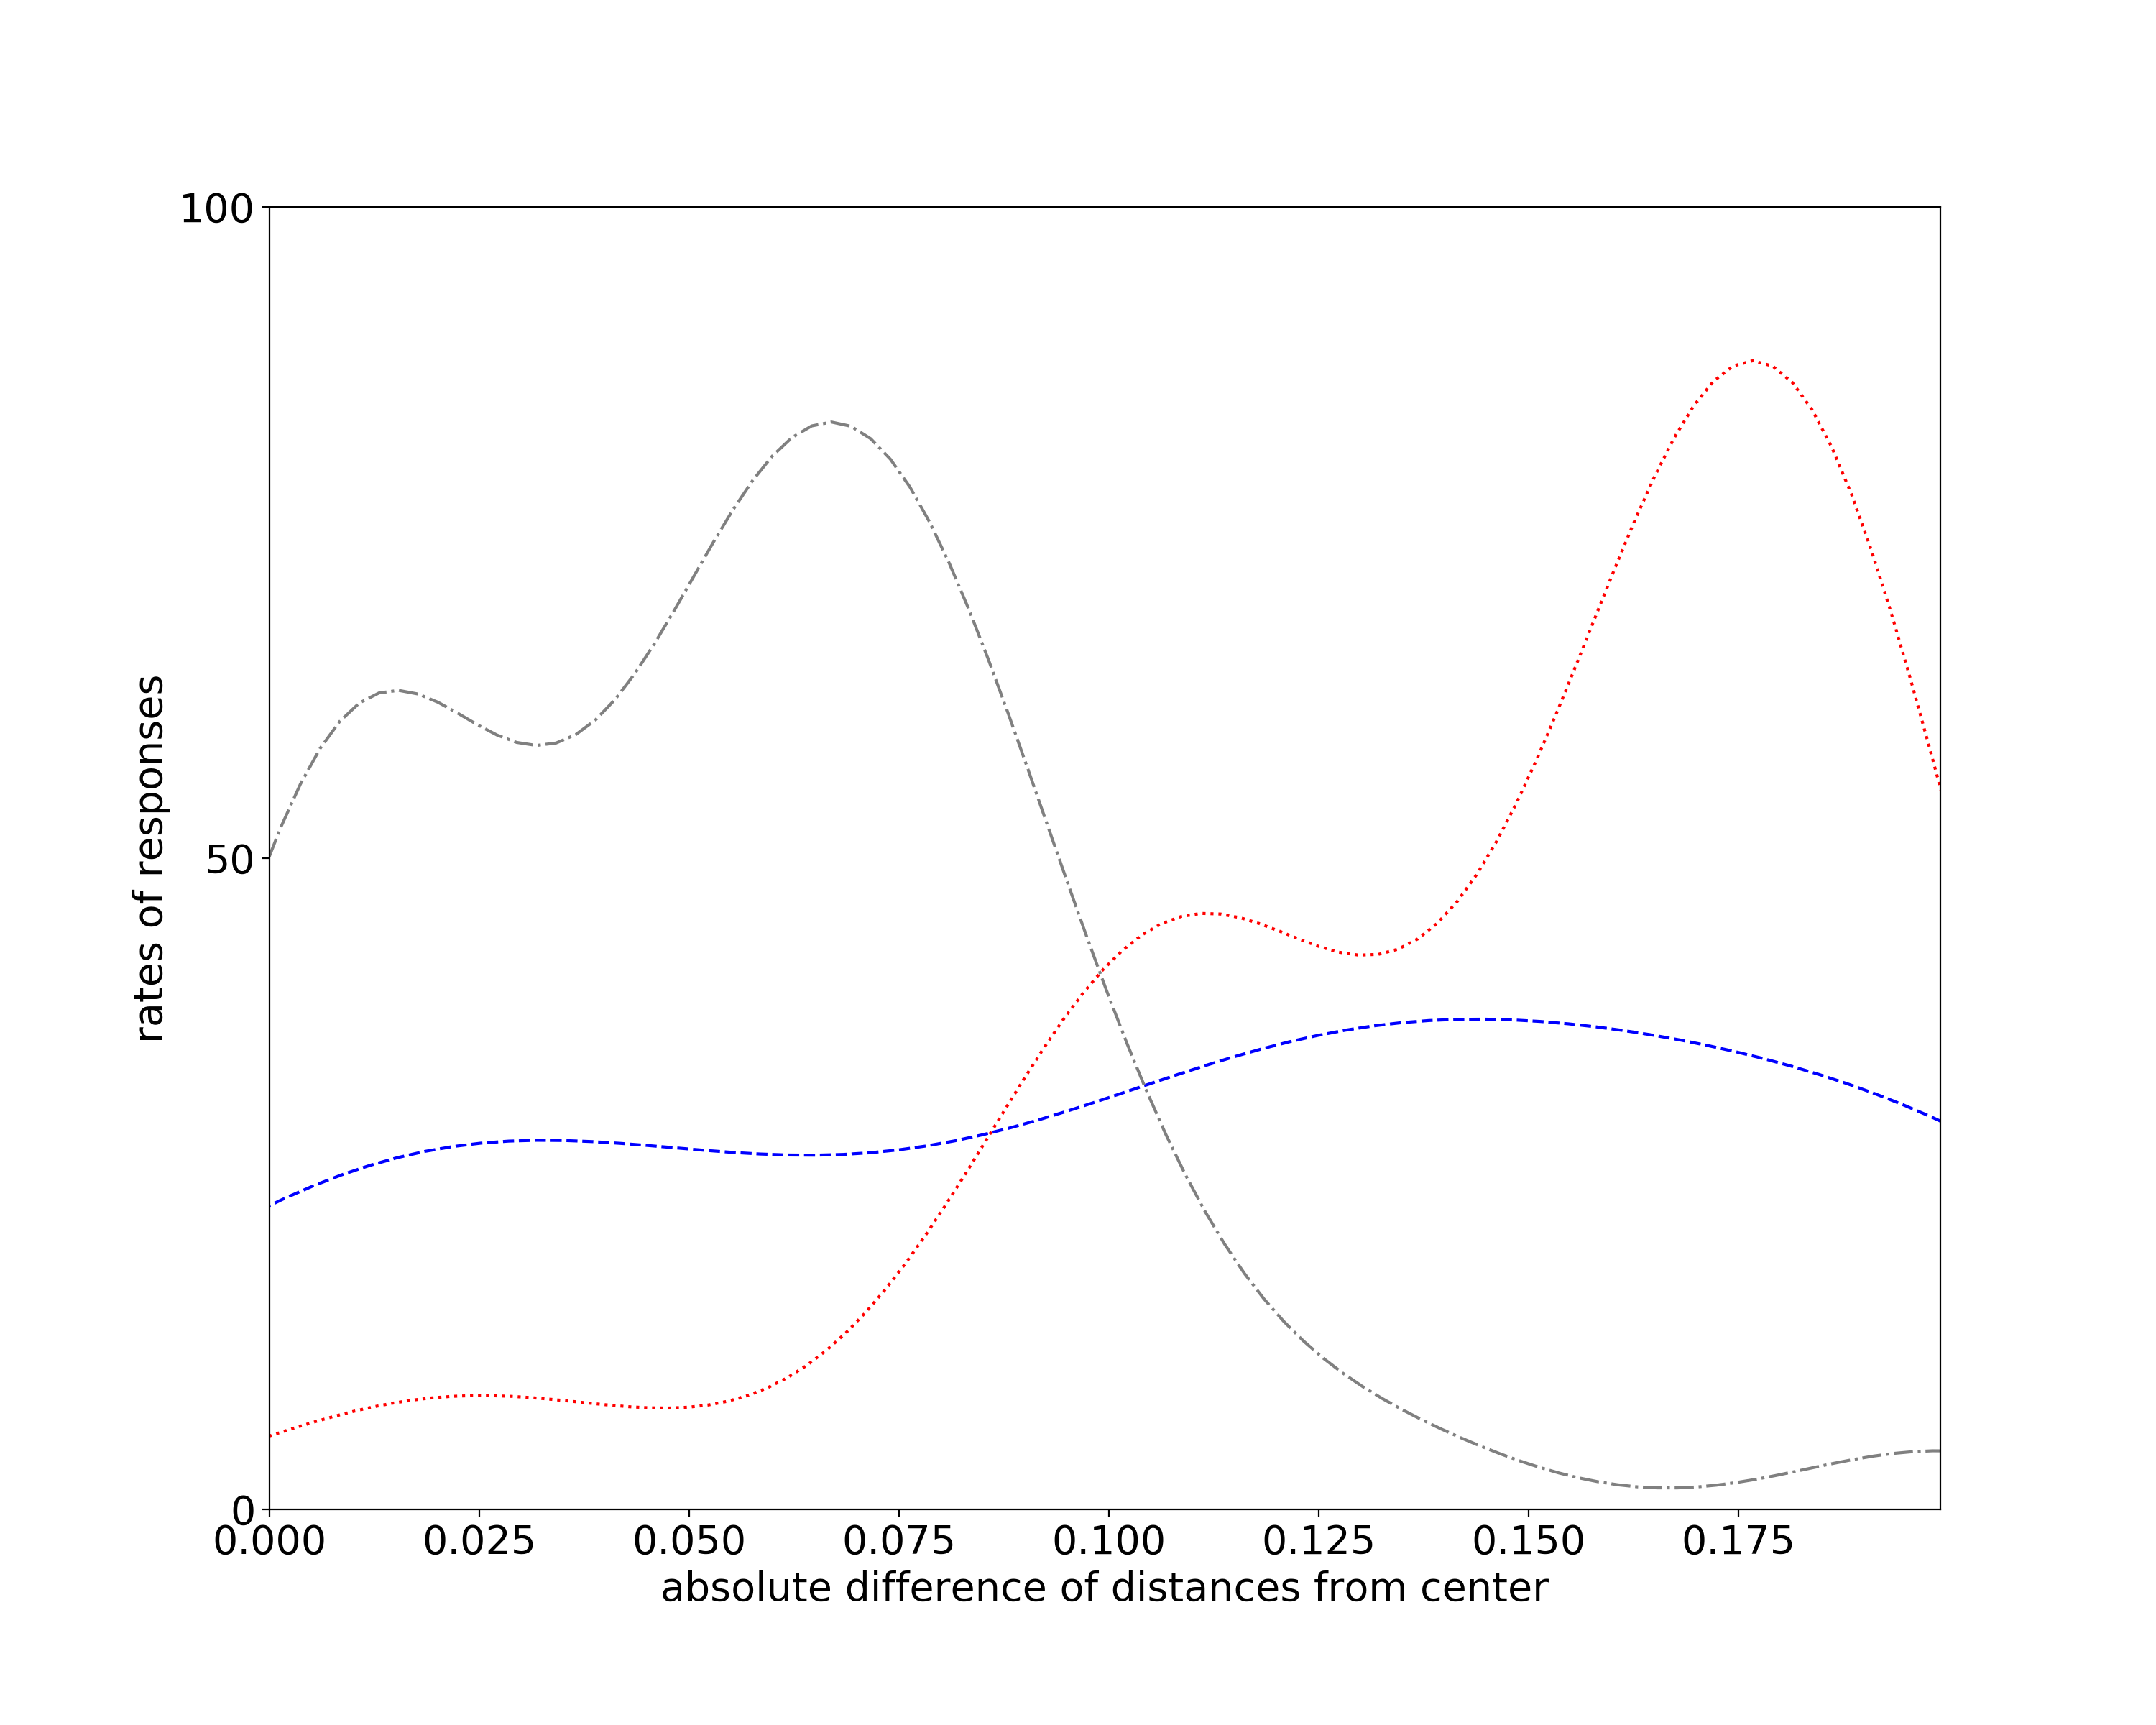
\includegraphics[height=0.23\textwidth]{cluttered-malihe.png}
    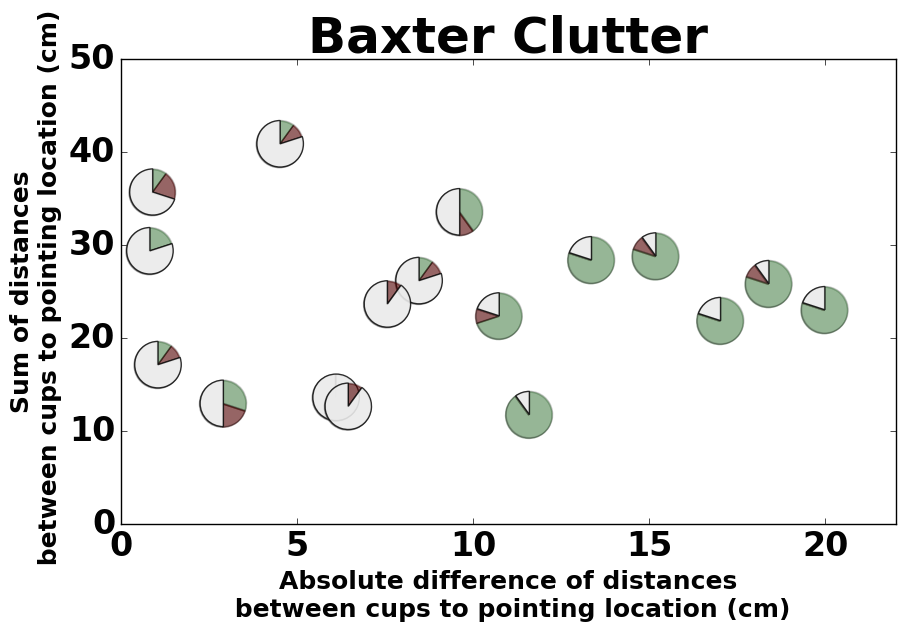
\includegraphics[width=\linewidth]{figures/baxter_Clutter_granular.png}
    % 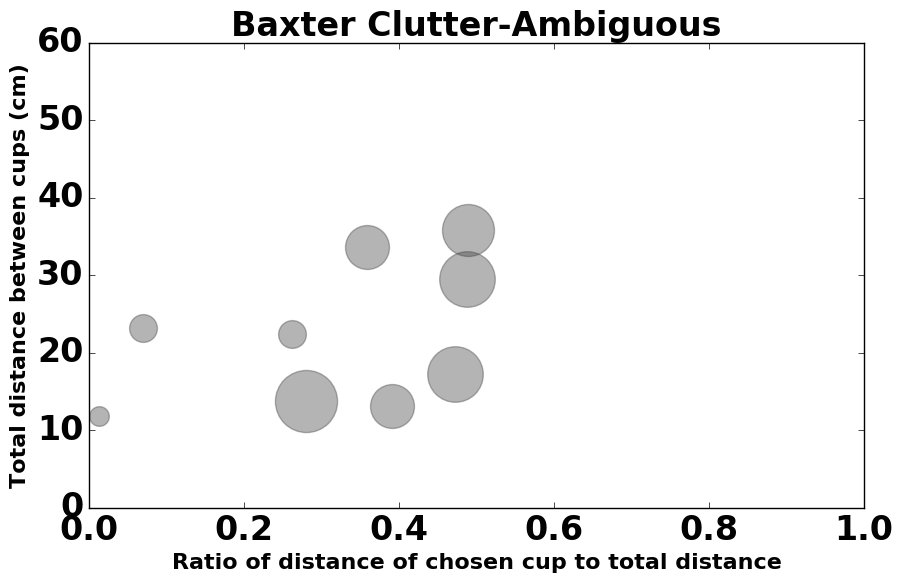
\includegraphics[width=0.35\textwidth]{figures/baxter_Clutter-Ambiguous2_granular.png}
    \caption{
    % (\textit{Top:} Histogram of responses in the cluttered scene. Red represents responses that correspond to the nearer object. Blue represents the farther object. Gray shows ambiguous responses. (\textit{Bottom:}) )
    The scatter plot represents the spread of responses where human subjects chose the \textit{nearer cup} (green), \textit{farther} cup (red), and ambiguous (grey). 
    The \textit{x-axis} represents the absolute difference between the distances of each cup to the locations of pointing, the \textit{y-axis} represents the total distance between the two cups.
    }
    \label{fig:cluttered}
\end{figure}

\paragraph{Different verbs}
The results of the Chi-squared test shows that in Spatial trials when we replace \textit{put} with \textit{place}, \textit{push} and \textit{move}, the differences of the distributions of \textit{correct}, \textit{incorrect} and \textit{ambiguous} responses are not statistically significant ($\chi=0.2344 $, $p = 0.971$). The coefficients of the multinomial logistic regression model and the p-values suggest that the differences in judgements for each sampled point with different verbs are not statically significant ($b<0.0001$ , $p>0.98$).



\paragraph{Cluttered}

% \begin{figure}[t!] what are those two blocks, give it we are going to attempt to come up with a principles that explain our observation
%     \centering
%     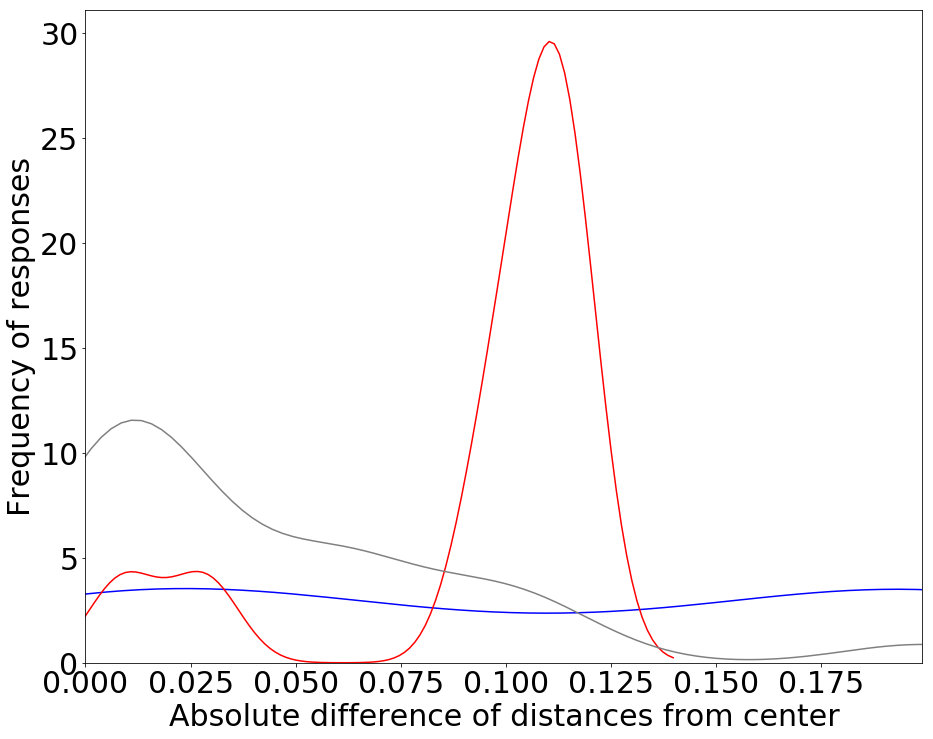
\includegraphics[width=0.3\textwidth]{figures/cluttered-histogram.png}
%     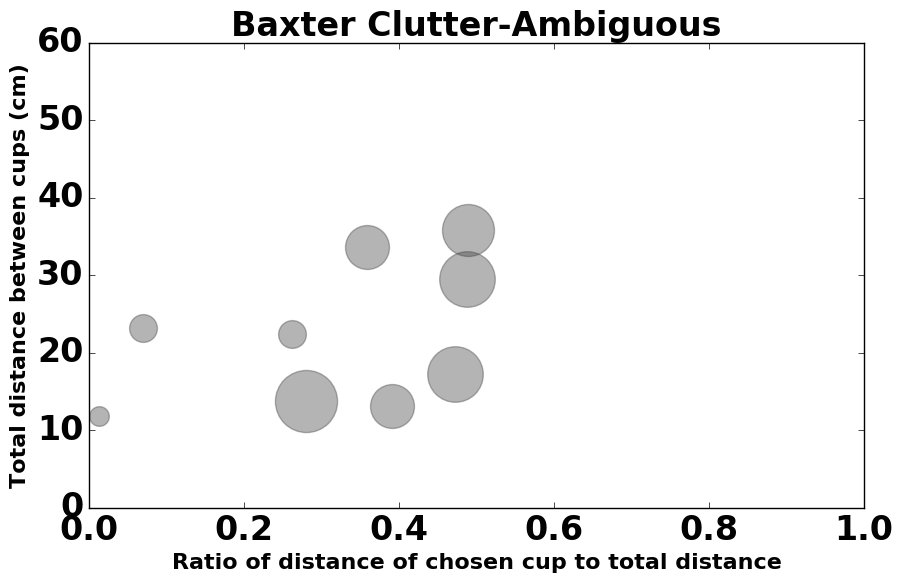
\includegraphics[width=0.35\textwidth]{figures/baxter_Clutter-Ambiguous2_granular.png}
%     \caption{(\textit{Top:} Histogram of responses in the cluttered scene. Red represents responses that correspond to the nearer object. Blue represents the farther object. Gray shows ambiguous responses. (\textit{Bottom:}) The scatter plot shows the ratio of the distance of a nearer object in an ambiguous response to the total distance, plotted against the total distance between objects. Most of these happen when the objects are too close to (close to the X axis), or equidistant from the pointing location (around the ratio of 0.5).)}
%     \label{fig:cluttered}
% \end{figure}



As we can see in Figure~\ref{fig:cluttered}, the higher is the absolute difference of centers of distances from the center, the more likely it is that subjects pick a mug (green or red) as opposed to the \textit{ambiguous} choice. That is when the two mugs were very close, almost next to each other (less than 10 cm apart), majority of subjects chose the \textit{ambiguous} option. 
 
% The blue line in Figure~\ref{fig:cluttered} shows the frequency of the cases 
% The red sections of the circles indicates responses
% when 

When the target is not very close to the distractor, and when the pointing finger points towards $x^*$ on the table that is closer to one mug, subjects picked the mug that was the correct target of the pointing action more often than the incorrect one. This was true for all of the cases in our dataset. Referential pointing is flexible. Even in the presence of a distractor, there is not need for accurate exact pointing, as long as the target object is not ambiguous, people interpret the pointing action correctly.






% \paragraph{speech}
% We study how varying the target of the pointing action from part of the space to a target object changes the interpretation of the pointing action by comparing the value of x* in each condition. $x^*$ represent the area on the table that contains the correct target of the pointing action. 



% To test our hypothesis, we will perform proportion test (two-tailed z-test) and the t-test in the exploratory analysis in case it is needed. 
% Another way to test this idea is through a logistic regression where the dependent variable is a binary variable indicating whether or not the pointing action is understood correctly, and the independent variable is $x^*$. In this regression framework, our hypothesis states that the coefficient of $x^*$ would be insignificant. 
% To study the values that $x^*$ can take, we randomly select 8 points in each quadrant in the circle that is the intersection of the cone that comes out of the index finger and the surface of the table.

  


% \begin{figure}
%     \centering
%     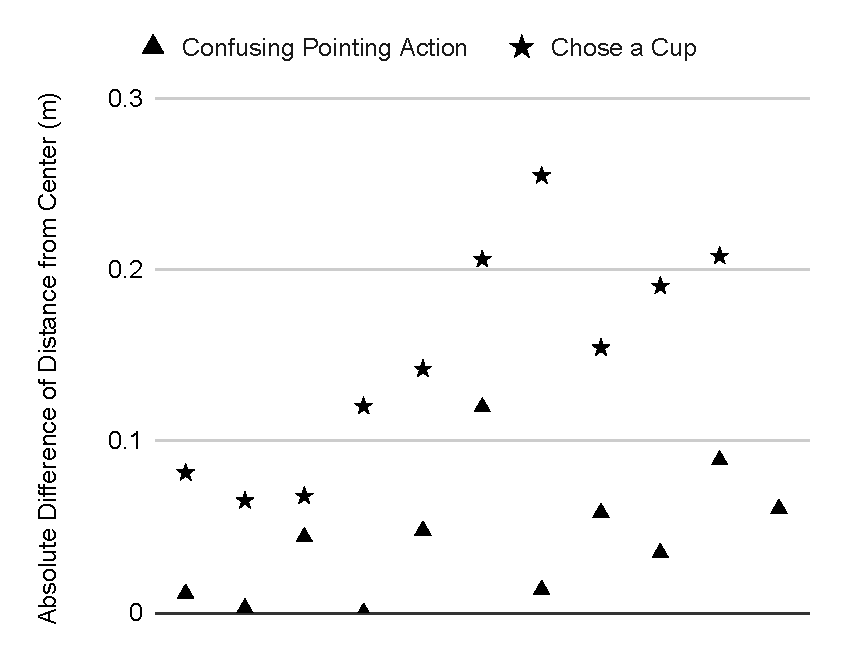
\includegraphics[width= \linewidth]{line_difference_chart (1).pdf}
%     \caption{Cluttered scene results}
%     \label{fig:line_figure}
% \end{figure}


% \begin{figure}
%     \centering
%     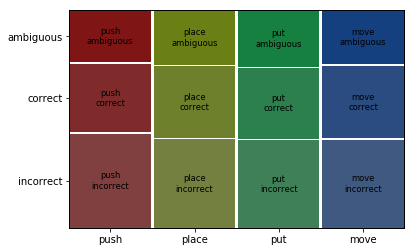
\includegraphics[width=\linewidth]{verbs.png}
%     \caption{different verbs}
%     \label{fig:verbs}
% \end{figure}



%  For instance in Figure~\ref{fig:aggregatesimple}, the 'correct' spatial responses are \textit{stretched} because of perspective. 
 
%  $ \epsilon = (\epsilon_1, \epsilon_2)$.
 


% \paragraph{Case 3: Referring expressions with pointing}

% $(x^*,RE), RE \subseteq \{ o_1, \dots, o_N \}  $ then \\
% Intended Object $= \argmin_{O \in RE} |O-x^*|$


% \paragraph{Case 3: Commonsense, Natural vs Unnatural}
% CS: constraints on possible interpretations of pointing action\\
% IR: Interpretation of pointing action= action of the addressee \\

% $IR \in CS$





